% Copyright 2004 by Till Tantau <tantau@users.sourceforge.net>.
%
% In principle, this file can be redistributed and/or modified under
% the terms of the GNU Public License, version 2.
%
% However, this file is supposed to be a template to be modified
% for your own needs. For this reason, if you use this file as a
% template and not specifically distribute it as part of a another
% package/program, I grant the extra permission to freely copy and
% modify this file as you see fit and even to delete this copyright
% notice. 


%%\documentclass[notes]{beamer}       % print frame + notes
%\documentclass[notes=only]{beamer}   % only notes
\documentclass{beamer}              % only frames


%\documentclass{beamer}
\usepackage{lmodern}
\usepackage{verbatim}
% There are many different themes available for Beamer. A comprehensive
% list with examples is given here:
% http://deic.uab.es/~iblanes/beamer_gallery/index_by_theme.html
% You can uncomment the themes below if you would like to use a different
% one:
%\usetheme{AnnArbor}
%\usetheme{Antibes}
%\usetheme{Bergen}
%\usetheme{Berkeley}
%\usetheme{Berlin}
%\usetheme{Boadilla}
%\usetheme{boxes}
%\usetheme{CambridgeUS}
%\usetheme{Copenhagen}
%\usetheme{Darmstadt}
%\usetheme{default}
%\usetheme{Frankfurt}
%\usetheme{Goettingen}
%\usetheme{Hannover}
%\usetheme{Ilmenau}
%\usetheme{JuanLesPins}
%\usetheme{Luebeck}
\usetheme{Madrid}
%\usetheme{Malmoe}
%\usetheme{Marburg}
%\usetheme{Montpellier}
%\usetheme{PaloAlto}
%\usetheme{Pittsburgh}
%\usetheme{Rochester}
%\usetheme{Singapore}
%\usetheme{Szeged}
%\usetheme{Warsaw}

\title[Master's Thesis]{Using Multiple Imputation, Survival Analysis, 
And Propensity Score Analysis In Cancer Data With A Large Amount Of Missing Data}

% A subtitle is optional and this may be deleted
\subtitle{Master's Thesis}

\author{Nathan Berliner \inst{1}}
% - Give the names in the same order as the appear in the paper.
% - Use the \inst{?} command only if the authors have different
%   affiliation.

\institute[Rice] % (optional, but mostly needed)
{
  \inst{1}%
  Department of Statistics\\
  Rice University
  }

\date{11/30/2015}
% - Either use conference name or its abbreviation.
% - Not really informative to the audience, more for people (including
%   yourself) who are reading the slides online

\subject{Statistics}
% This is only inserted into the PDF information catalog. Can be left
% out. 

% If you have a file called "university-logo-filename.xxx", where xxx
% is a graphic format that can be processed by latex or pdflatex,
% resp., then you can add a logo as follows:

% \pgfdeclareimage[height=0.5cm]{university-logo}{university-logo-filename}
% \logo{\pgfuseimage{university-logo}}

% Delete this, if you do not want the table of contents to pop up at
% the beginning of each subsection:
\AtBeginSubsection[]
{
  \begin{frame}<beamer>{Outline}
    \tableofcontents[currentsection,currentsubsection]
  \end{frame}
}

% Let's get started
\begin{document}

\begin{frame}
  \titlepage
\end{frame}

\begin{frame}{Outline}
  \tableofcontents
  % You might wish to add the option [pausesections]
\end{frame}

% Section and subsections will appear in the presentation overview
% and table of contents.
\section{Introduction}
\subsection{The Problem}

%\subsection{}

\begin{frame}{In an ideal world}
  \begin{itemize}
  \item We would have a large dataset
  \begin{itemize}
   \item That was obtained from an RCT
   \item That would help answer a clearly defined question
   \item That had all the covariates of scientific interest
   \item That contained no missing data
  \end{itemize}

  \end{itemize}
\end{frame}

\begin{frame}{In Reality}

  \begin{itemize}
   \item RCT's are expensive and often unethical
   \begin{itemize}
    \item We often get retrospective observational data
    \item Pulled from a database or historical records
   \end{itemize}

   \item The questions we have may not be answerable from the data on hand
   \begin{itemize}
    \item The data obtained often doesn't support the original question in mind
   \end{itemize}

   \item The covariates collected are out of our control
   \begin{itemize}
    \item Since often no control of experiment, no control over what is collected
   \end{itemize}

   \item Lots of missing data
   \begin{itemize}
    \item Since no control over how the data is collected, we can't guarantee that everything is collected
   \item This issue is seemingly omnipresent in all types of data collection
   \end{itemize}

  \end{itemize}
  \note{hey!}

\end{frame}

\begin{frame}{Is This a Problem?}

  \begin{itemize}
   \item Without an RCT, we can't be sure if differences in treatments is due to the treatment or something else
   \item Omitting important factors may bias our results
   \item With missing data, we will be throwing away data and biasing our results
  \end{itemize}


\end{frame}

\begin{frame}{The Solution}
This thesis aims to fix some of these problems
  \begin{itemize}
   \item Fill in missing data via multiple imputation
   \item Create meaningful analytical models via survival analysis
   \item Get a causal interpretation from observational data
  \end{itemize}


\end{frame}

\begin{frame}{Motivation}
\begin{itemize}
   \item This thesis is motivated by cancer survival data with moderate missingness
   \item We will build the theory for dealing with this sitation
   \item And then apply it to a cancer data set
  \end{itemize}


\end{frame}

\begin{frame}{Abstract}
In this thesis, multiple imputation, survival analysis, and propensity score analysis are combined in 
order to answer questions about cancer data with moderate missingness. While each of these fields have 
been studied individually, there has been little work and analysis on using the three in trio.
Starting with an incomplete dataset, we aim to impute the missing data, run survival analysis on each
of the imputed datasets, and then do propensity score analysis to observe causal effects.
Along the way, many theoretical and analytical decisions are mode. I explain why each decision is made, 
and offer ample evidence for the other choices such that the interested reader may implement the methods
if they so choose. I apply the methodology to a cancer survival dataset in a case study, but the methods 
used are general, and could be adapted for any type of data.
 
\end{frame}

\subsection{Missing data}
\begin{frame}
 \begin{itemize}
 \item Missing data happens when we intend to collect a piece of data but don't actually get it
 \item Historical approaches
 \begin{itemize}
  \item Complete Case analysis: Throw away any record that is not complete
  % list of downsides
 \item Available Case analysis: Use records so long as they are complete for the specific analysis in question
 %bad things here
 \end{itemize}
 \end{itemize}
\end{frame}


\begin{frame}{Imputation}
\begin{block}{Definition}
The English verb ``to impute'' comes from the Latin imputo, which means
to reckon, attribute, make account of, charge, ascribe. \cite{VanBuuren2012}
\end{block}
\begin{itemize}
 \item In the 1930's, Allan, Wishart,and Yates laid framework for missing data
 \begin{itemize}
  \item Idea: Fill in the missing value, deduct degrees of freedom to account for it
  \item Issue: Dogmatic, and variance can't be estimates correctly
 \end{itemize}

\end{itemize}

 
\end{frame}

\begin{frame}{Multiple Imputation}
Throughout the 70's and 80's Donald Rubin worked to improve on this
\begin{itemize}
 \item Instead of imputing one value, lets impute it $m\geq 2$ times
 \item Draw the values from the missing datas posterior distibution given the observed
 data and the process that generated the missing data
\end{itemize}
This idea is called Multiple Imputation (MI) and was formalized in 1987 \cite{Rubin1987}. It is the gold standard method
for missing data currently.
\end{frame}


\begin{frame}{How does MI work?}
 \begin{figure}[h!]
  \centering
    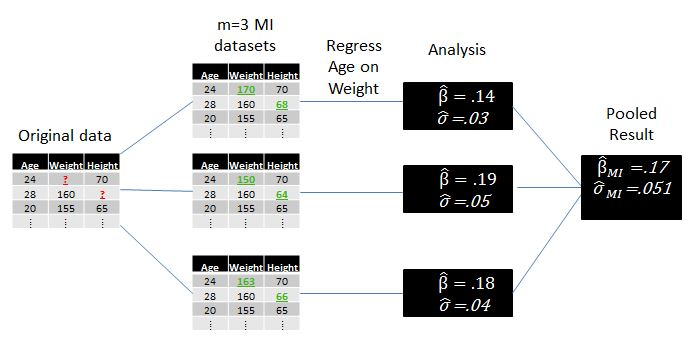
\includegraphics[width=0.8\textwidth]{mi_example_full.jpg}
  \caption{Visualization of MI data}
\label{fig:miexample}
\medskip
\small
Missingness is displayed by \textcolor{red}{?'s} and the imputed data is shown  as \textcolor{green}{\#'s}.
We then regress age on weight, get the results from the individual datasets, and then pool them together.
\end{figure}
\note{We will go in to much more detail later in presentation}
\end{frame}



\subsection{Survival Analysis}

\begin{frame}{Survival Analysis}
\begin{block}{Survival Analysis}
Survival analysis is a field of statistics concerned with analyzing time to 
event data, often in the face of censoring or truncation.
\end{block}
Examples:
\begin{itemize}
 \item The survival of patients after a liver transplant in a hospital
 \begin{itemize}
  \item Complications: study ending, patients die before study starts, subject moves away
 \end{itemize}

 \item The time until a child learns a new task
 \begin{itemize}
  \item Complications: refuse participation, move away, don't recall the exact time they learned,
  already learned the task
 \end{itemize}

\end{itemize}
\end{frame}

\begin{frame}{Kaplan-Meier Estimator}
\begin{itemize}
 \item The survival function $S(t)=P(T>t)=\int_{t}^{\infty}f(u)du$ is estimated by the 
 nonparametric Kaplan-Meier Estimator
 $$\hat{S}(t)=\prod_{t_i<t}\frac{n_i -d_i}{n_i}$$
\item $n_i$ is the number of subject in the risk set at time $t_i$
\item $d_i$ is the number of deaths at time $t_i$
\end{itemize}
\note{We use death and survival because easy to say, but it really means event or not}
\end{frame}

\begin{frame}{Log rank test}
The log rank test compares two survival curves to see if from the same distribution

$$\frac{\sum_{j=1}^{J}w_j(O_{1j}-E_{1j})}{\sqrt{\sum_{j=1}^{j}w_j^2V_{j}}}\sim N(0,1)$$
\begin{itemize}
 \item Where $w_j$ is the weight of each observation (must be $\geq 0$, we will set all to be 1)
 \item $N_j=N_{1j}+N_{2j}$ is the number at risk at time j (composed from deaths in each group)
 \item $O_j=O_{1j}+O_{2j}$ is the observed number of deaths at time j (composed from the observed deaths in each group)
 \item $E_{1j}=\frac{O_jN_{1j}}{N_j}$
 \item $V_j=\frac{O_j(N_{1j}/N_j)(1-N_{1j}/N_j)(N_{j}-O_{j})}{N_j -1}$
 \end{itemize}
\note[itemize]{Weights such as

\item peto peto
\item gehan

will put emphasis on different parts of the survival curve
}
\end{frame}


\begin{frame}{Cox Regression}
%might want to use the underbraces
%$\underbrace{h_{0}(t)}_{\textrm{time}}*\underbrace{exp(\sum_{k=1}^{p}\beta_{k}Z_{k})}_{\textrm{covariates}}$
\begin{itemize}
 \item Hazard is the instantaneous rate of event given that you have survived until time t, given 
 by $$h(t)=\lim_{\Delta t \rightarrow 0+}\frac{P[t\leq T<t+\Delta t|T\geq t]}{\Delta t}$$
   \item Cox regression models hazard by 
   
   %$$h(t|Z)=h_{0}(t)\exp(\sum_{k=1}^{p}\beta_{k}Z_{k})$$
   $$h(t|Z)=\underbrace{h_{0}(t)}_{\textrm{time}}*\underbrace{exp(\sum_{k=1}^{p}\beta_{k}Z_{k})}_{\textrm{covariates}}$$

   \item Where $h_{0}(t)$ is the baseline hazard
   \item $Z_k$ is the $k^{th}$ covariate
   \item $\beta_k$'s are found by maximizing the partial likelihood function
 \end{itemize}
The covariates act to multiply the hazard function.
\end{frame}

\subsection{Causal Analysis}
\begin{frame}{Causal Analysis}
Suppose we have a new drug we want to test to see how efficacious it is.
 \begin{itemize}
  \item We would like to be able to say ``The drug leads to better health''
  \begin{itemize}
   \item But need an RCT to say this
   \item We only have observational data
   \item Thus differences could be attributed to the drug or another factor (like healthier people
   decided to take the drug)
  \end{itemize}
Idea: try to balance the covariates so the two groups seem identical at baseline
 \end{itemize}

\end{frame}

\begin{frame}{Counterfactual Model}
\begin{itemize}
 \item Suppose that for or every person, there are two potential outcomes
 \begin{itemize}
  \item $Y_i(0)$ - The outcome if they had taken the control
  \item $Y_i(1)$ - The outcome if they had taken the treatment
 \end{itemize}
\item Obviously, we only observe one. The fundamental problem of causal inference
\item If we could observe both, then we could observe the causal effects for each person
\item We will have to settle for finding the average treatment effect (ATE)
\end{itemize}
 
\end{frame}

\begin{frame}{Propensity scores}
\begin{block}{Definition}
The propensity score is the probability that the subject received the treatment given the subjects
covariates. It is computed using the patient's baseline (pretreatment) information \cite{Rosenbaum1983}
\end{block}
 \begin{itemize}
  \item Assume that the covariates play a role in how the subject chose treatment
  \item Controling for propensity score will make groups seem indistinguishable
  \item Thus, we may treat it as if it were an RCT
 \end{itemize}

\end{frame}

\begin{frame}{Common Propensity Score Methods}
\begin{itemize}
 \item Matching: Match treatment and controls on their propensity score, calculate ATE
 \item Stratification: Stratify on propensity score, weight and combine ATE in each strate
 \item Weighting: Weight each observation by the inverse of its propensity score, and then calculate ATE
\end{itemize}

 
\end{frame}

% You can reveal the parts of a slide one at a time
% with the \pause command:
\begin{frame}{Second Slide Title}
  \begin{itemize}
  \item {
    First item.
    \pause % The slide will pause after showing the first item
  }
  \item {   
    Second item.
  }
  % You can also specify when the content should appear
  % by using <n->:
  \item<3-> {
    Third item.
  }
  \item<4-> {
    Fourth item.
  }
  % or you can use the \uncover command to reveal general
  % content (not just \items):
  \item<5-> {
    Fifth item. \uncover<6->{Extra text in the fifth item.}
  }
  \end{itemize}
\end{frame}

\section{Second Main Section}

\subsection{Another Subsection}

\begin{frame}{Blocks}
\begin{block}{Block Title}
You can also highlight sections of your presentation in a block, with it's own title
\end{block}
\begin{theorem}
There are separate environments for theorems, examples, definitions and proofs.
\end{theorem}
\begin{example}
Here is an example of an example block.
\end{example}
\end{frame}

% Placing a * after \section means it will not show in the
% outline or table of contents.
\section*{Summary}

\begin{frame}{Summary}
  \begin{itemize}
  \item
    The \alert{first main message} of your talk in one or two lines.
  \item
    The \alert{second main message} of your talk in one or two lines.
  \item
    Perhaps a \alert{third message}, but not more than that.
  \end{itemize}
  
  \begin{itemize}
  \item
    Outlook
    \begin{itemize}
    \item
      Something you haven't solved.
    \item
      Something else you haven't solved.
    \end{itemize}
  \end{itemize}
\end{frame}



% All of the following is optional and typically not needed. 
\appendix
\section<presentation>*{\appendixname}
\subsection<presentation>*{For Further Reading}
\begin{comment}
 

\begin{frame}[allowframebreaks]
  \frametitle<presentation>{For Further Reading}
    
  \begin{thebibliography}{10}
    
  \beamertemplatebookbibitems
  % Start with overview books.

  \bibitem{Author1990}
    A.~Author.
    \newblock {\em Handbook of Everything}.
    \newblock Some Press, 1990.
 
    
  \beamertemplatearticlebibitems
  % Followed by interesting articles. Keep the list short. 

  \bibitem{Someone2000}
    S.~Someone.
    \newblock On this and that.
    \newblock {\em Journal of This and That}, 2(1):50--100,
    2000.
  \end{thebibliography}
\end{frame}
\end{comment}

\begin{frame}[allowframebreaks]
        \frametitle{References}
        \bibliographystyle{ieeetr}
	\bibliography{Research}
\end{frame}
\end{document}


